\section{System's Perspective} 

\subsection{MiniTwit Application}
We chose to rewrite MiniTwit to C\# to utilize Blazor WebAssembly, which allows us to write all code in the same language \autocite{dotnetblazor, dotnet}. Blazor additionally runs as a single-page application which is faster at loading, partly because data can be fetched in the background and because full-page reloads are rare. One downside of WebAssembly is the long initial load of the application, which hopefully can be reduced or removed with future versions of DotNet.
Our application depends on some NuGet packages to communicate with the rest of the system \autocite{nuget}.

\begin{center}
\begin{tabular}{|c|p{0.6\linewidth}|}
    \hline
    Identity Server & An easy and secure way of managing users \autocite{duendeidentityserver}. \\
    \hline
    Prometheus-net & Sets up the  /metrics endpoints for Prometheus. \\
    \hline
    Serilog.Sinks.ElasticSearch & Gives Serilog a log sink for ElasticSearch, letting it send logs directly to ElasticSearch \\
    \hline
    EF Core & O/RM for communicating with the database\\
    \hline
\end{tabular}
\end{center}


We aimed for our system to have a simple and maintainable architecture, by utilizing as few different tools as possible and by striving to follow some architectural patterns. These were Clean Architecture, Repository Pattern, and Client-Server \autocite{clean-architecture, repository-pattern, client-server-architecture}. 

\texttt{Clean architecture} gives us separation of concern and greater modularity. We achieve this by having our code split into 4 C\# projects:

\begin{wrapfigure}{r}{0.4\textwidth}
    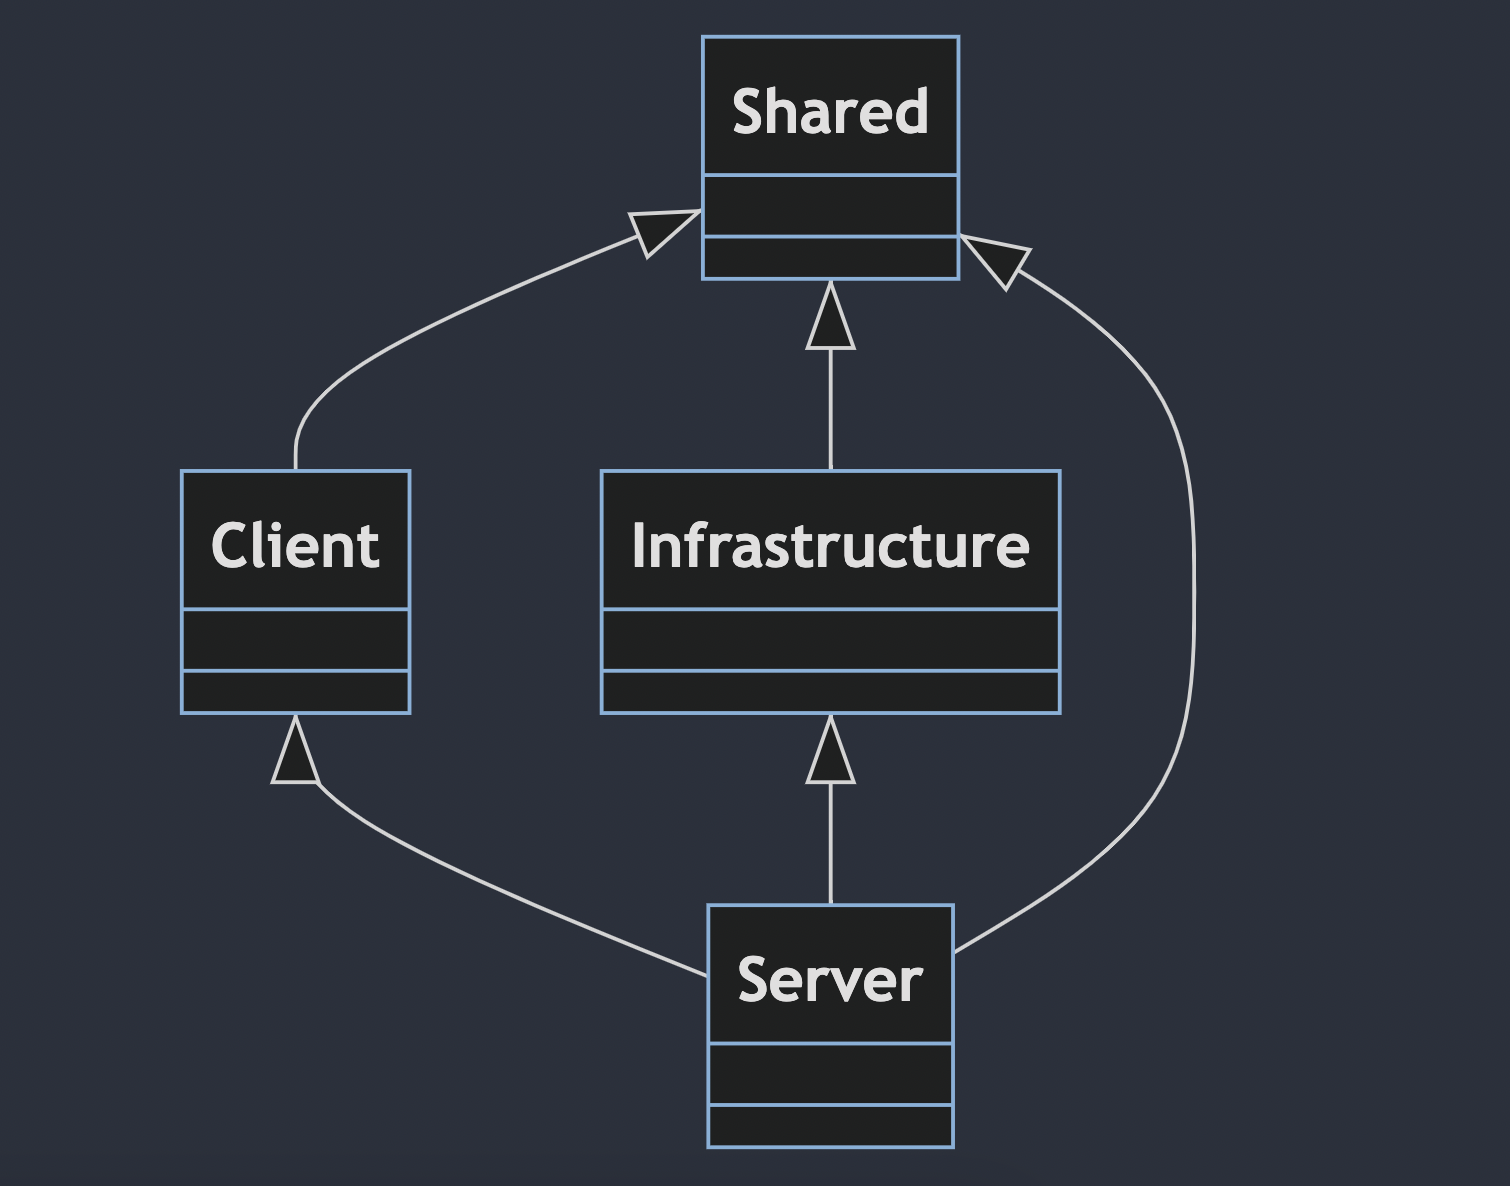
\includegraphics[width=0.9\linewidth]{Images/onionStructure.png} 
    \caption{Project Architecture}
    \label{fig:projectDependencyGraph}
\end{wrapfigure}

\begin{itemize}
    \item \texttt{Shared}
    \item \texttt{Infrastructure}
    \item \texttt{Client}
    \item \texttt{Server}
\end{itemize}

\texttt{Shared} is for our data transfer objects (\texttt{DTO's}) and repository interfaces, so we will be able to mock our repositories without a dependency on them. \texttt{Infrastructure} is for the repositories, database context, and models for the database schema, where the repositories depend on \texttt{Shared}. \texttt{Client} contains the \texttt{Blazor} files responsible for the presentation layer and user interface. \texttt{Server} is the actual server that contains the API controllers, application configuration, and serves the frontend. The controllers depend on \texttt{Infrastructure} and \texttt{Shared}, as the controllers need the repositories and the DTO's. For the \texttt{Server} to serve the frontend it depends on the \texttt{Client}. Thus none of our projects are mutually dependent and \texttt{Shared} is the core, from where it aggravates outward to a layer containing \texttt{Infrastructure} and \texttt{Client}. Lastly a layer containing \texttt{Server} as the part that other systems interacts with.

We use a \texttt{Repository pattern} to add abstraction around our communication with the database. Even though we use EF Core which some would say is enough abstraction, then repositories allow us to make a switch over to use something like \texttt{Dapper} instead of \texttt{EF Core} \autocite{dapper, efcore}.

\subsubsection{API Request Route}
The route of data in our application starts when a user sends a request to the server. It will then pass through a few places before it returns. Below is a sequence diagram illustrating the journey of an arbitrary request along its designated 'route'.

\vspace{3pt}
\begin{figure}[H]
    \centering
    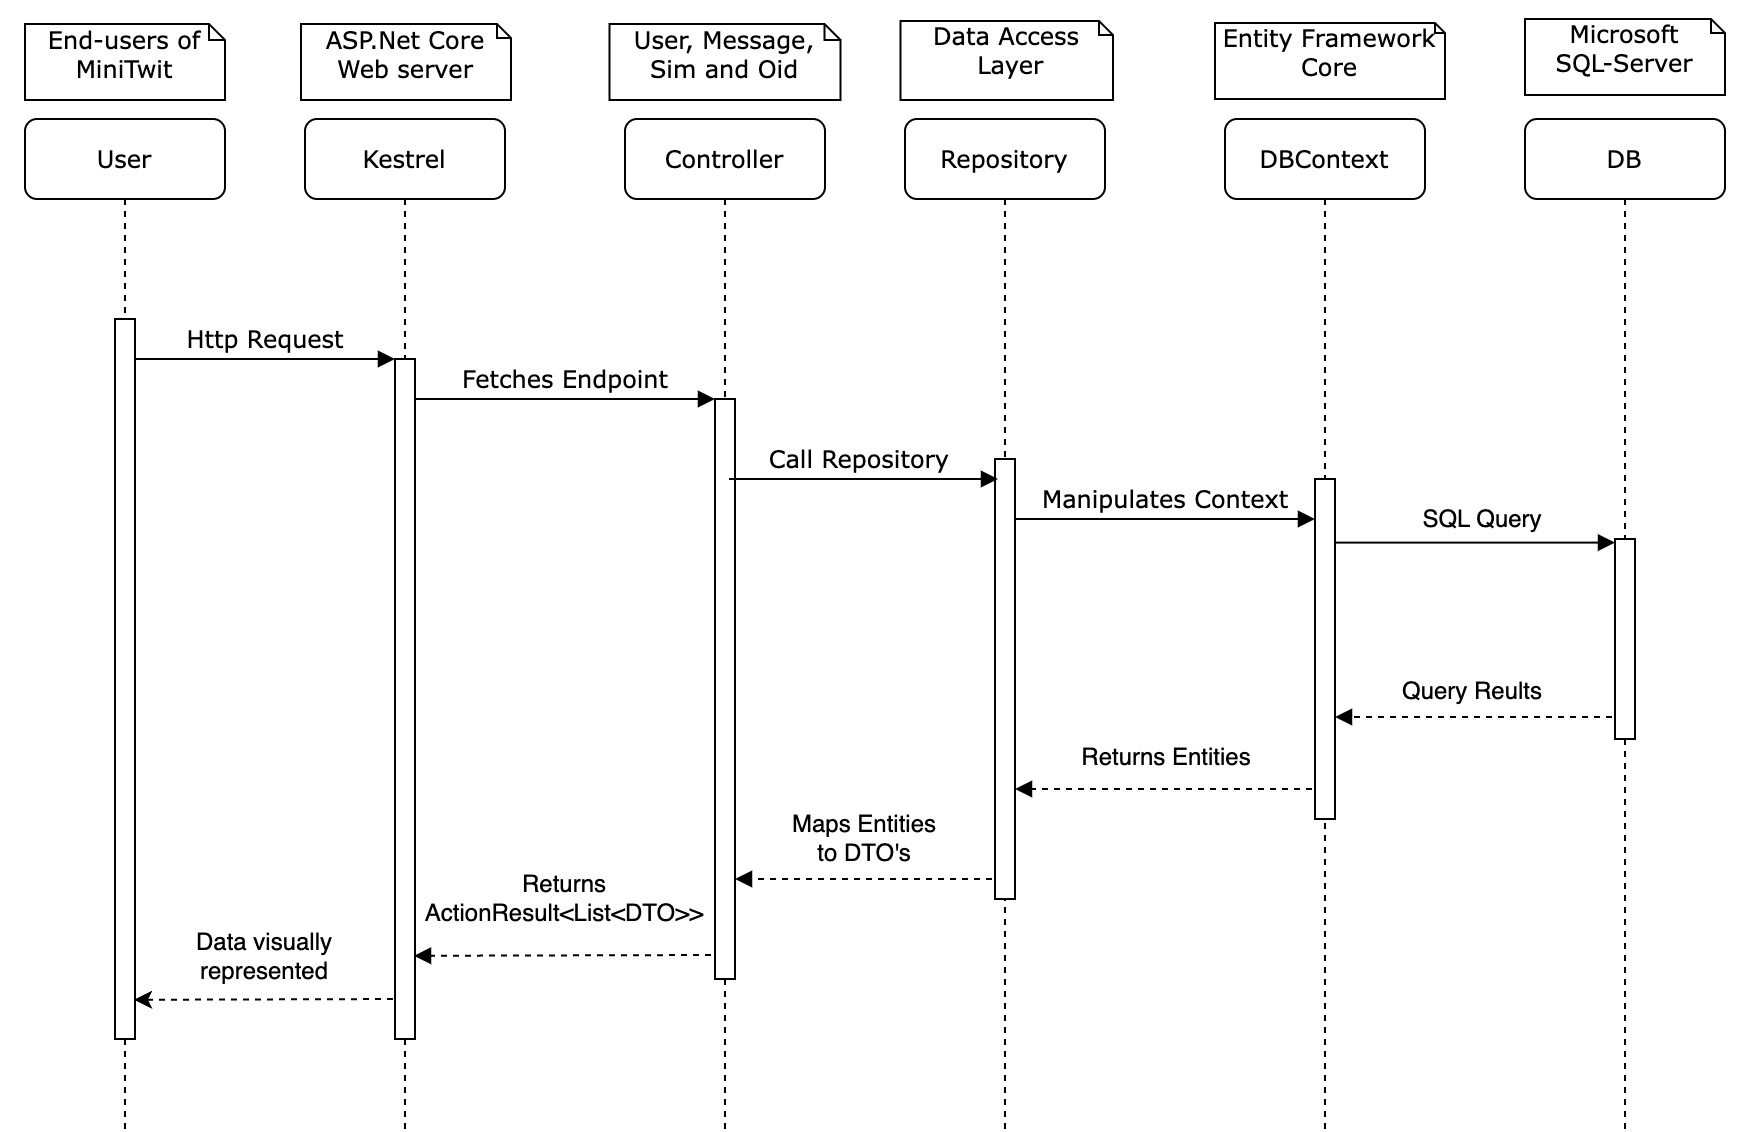
\includegraphics[width=0.65\linewidth]{Images/SequenceDevOps.jpg} 
    \caption{Data journey}
    \label{fig:API_Sequence}
\end{figure}
\vspace{3pt}

After a user sends a request, the server (Kestrel) receives it and sends it to the controller method that matches the endpoint that was targeted. The controller then uses one of the repositories that asks EF Core to format a query and send it to the database. The database then returns the data in the opposite sequence, until it reaches the user again.

\subsubsection{Database}
\noindent For communication between server and database, we chose the popular open-source O/RM Entity Framework Core, also known as EF Core, that makes it possible to define the database schemas and maintain the database state. Additionally, it removes the type barriers between code and database. This makes it possible to query the database without writing SQL, which blocks SQL injection.

\subsubsection{Dependencies}
At a low abstraction level, our application has specific dependencies such as libraries and packages. These are imported and installed using dotnet as the NuGet package manager. A visual representation can be seen in figure \ref{fig:packageDependencyGraph}. 

\begin{figure}[H]
    \centering
    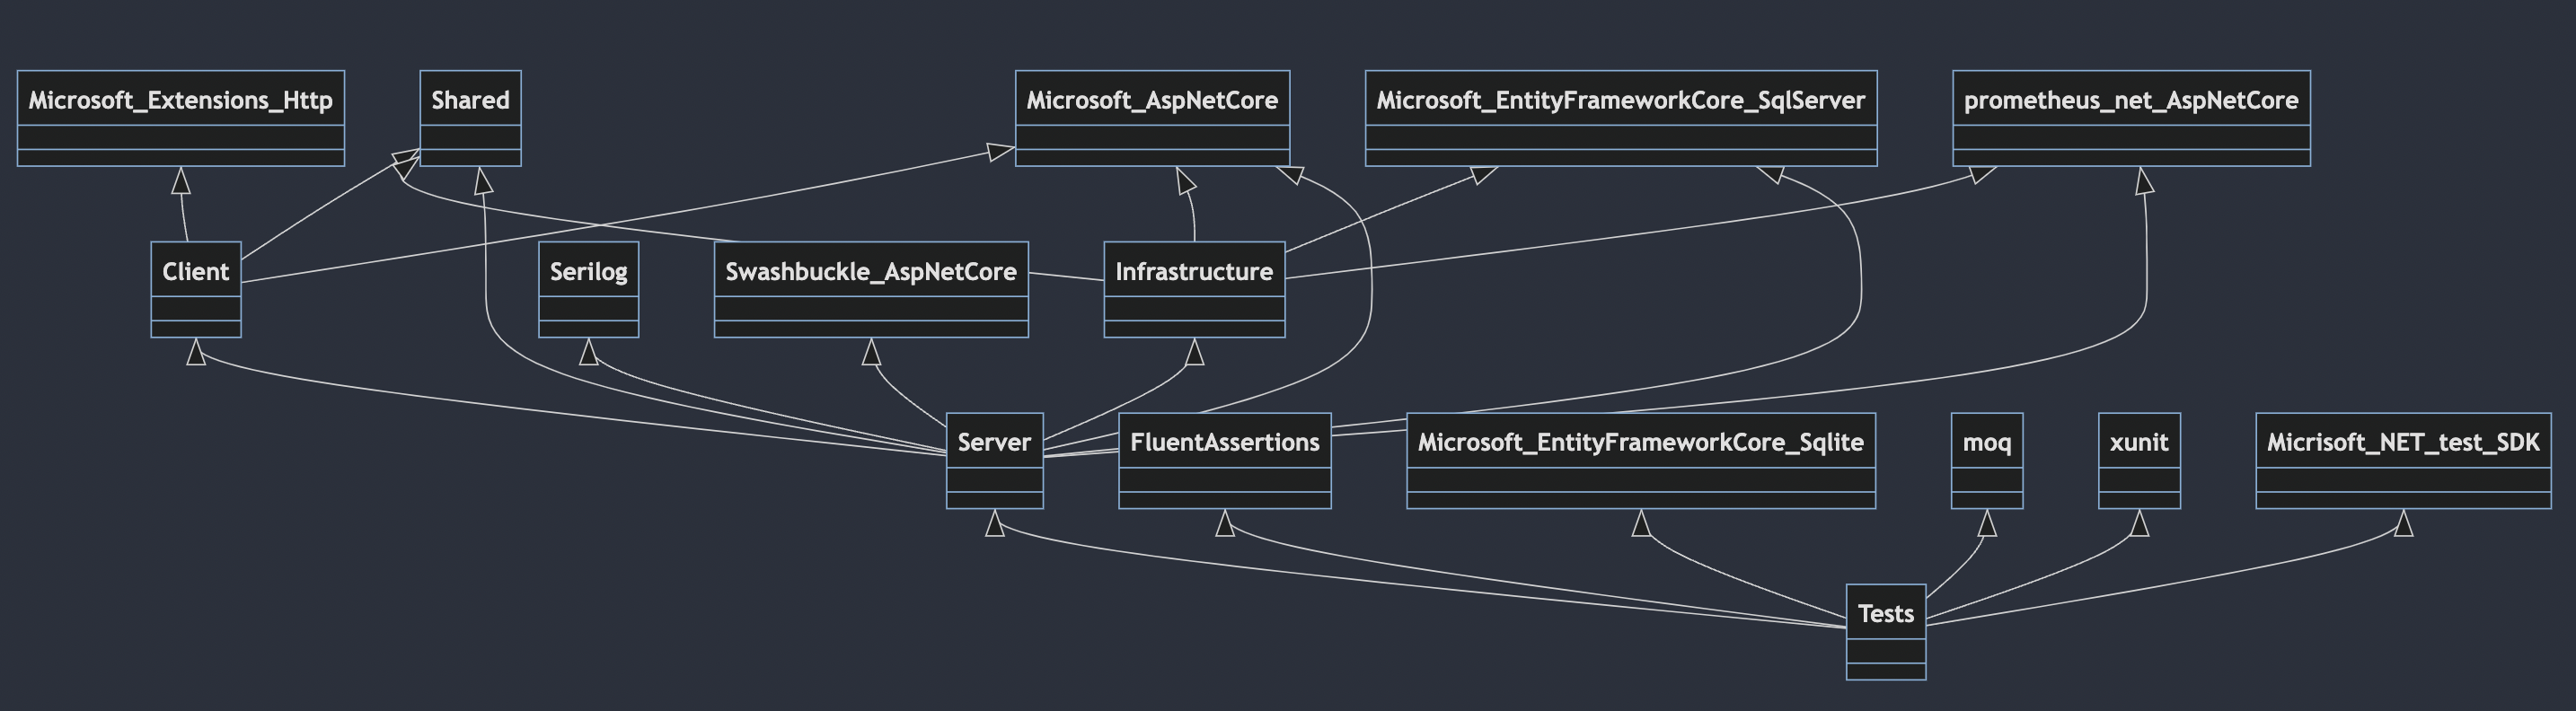
\includegraphics[width = \textwidth]{Images/dependencies2.png}
    \caption{Package dependency graph for C\# application}
    \label{fig:packageDependencyGraph}
    \centering
\end{figure}

\subsection{Tools \& Expanded System Architecture}

This section briefly describes the different tools used and their purpose. Most are expanded upon in the Process Perspective section. Figure \ref{fig:infrastructureDependencyGrapg} shows an overview of the infrastructure and dependencies of the system and its tools. 

\begin{figure}[H]
    \centering
    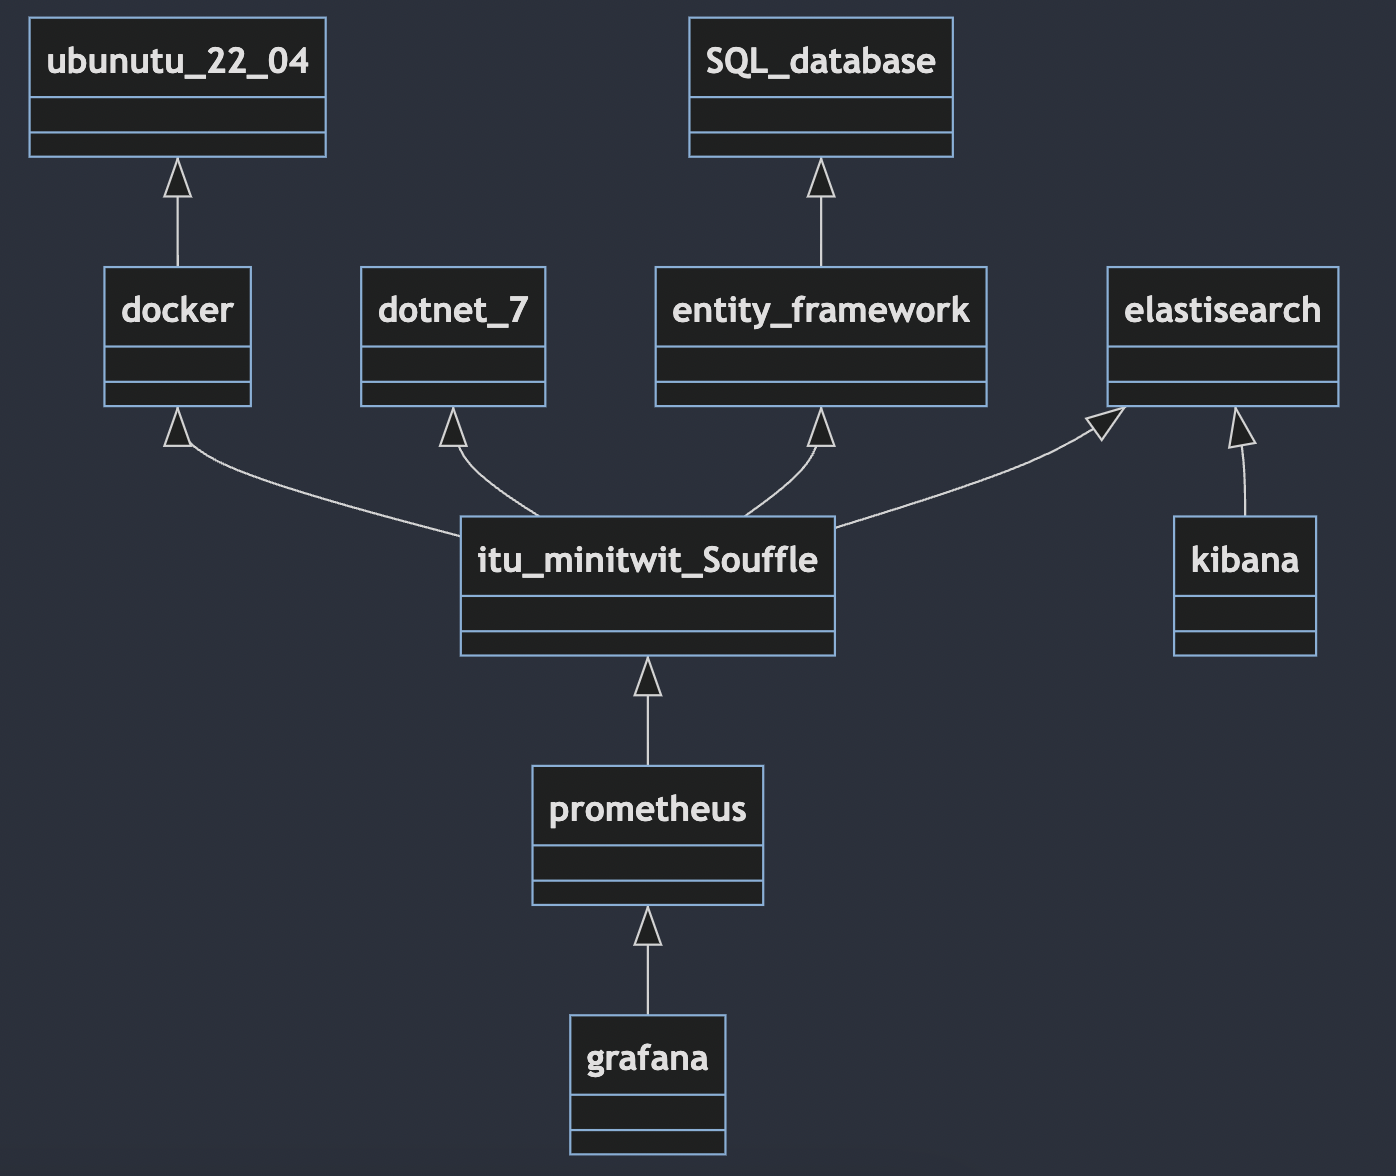
\includegraphics[width = 0.6\textwidth]{Images/application_dependencies.png}
    \caption{Infrastructure dependency graph}
    \label{fig:infrastructureDependencyGrapg}
    \centering
\end{figure}


\subsubsection{.NET 7}
This is the platform our project is built on. We chose this runtime since it's the one we are most familiar with and it contains a lot of libraries that suit our needs.

\subsubsection{Docker \& Ubuntu 22.04}
Docker is responsible for building, shipping, and running our application through containers \autocite{docker}. It makes it possible to have complete control of the environment in which the programs must run (we use Ubuntu 22.04). This ensures compatibility and portability; all it needs to run is the docker engine. Docker Swarm also enables scaling of the system within virtual machines \autocite{docker-swarm}.

\subsubsection{Digital Ocean}
As recommended, Digital Ocean is our chosen provider of cloud infrastructure. It's user-friendly and makes controlling our domain name simple by allowing it to be routed through Digital Oceans NS records \autocite{digitalocean}. However, as providers go, it's expensive. We had limited free credits and were restricted in the number of virtual machines we could afford. Our system has two droplets; one for our server, and one for all our tools. We would have preferred to separate our tools on individual droplets, potentially managed as a swarm for easy balancing.

\subsubsection{GitHub Actions}
GitHub Actions allows us to integrate our workflows, and apply our tools and tests to our branches before merging them together, ensuring a certain level of quality control \autocite{github-actions}.

\subsubsection{Prometheus \& Grafana}
Prometheus is responsible for monitoring our system by periodically querying its specified metric endpoints for data \autocite{prometheus}. This data is then accessed by Grafana, which is the platform responsible for visualizing it on its dashboards \autocite{grafana}. See \ref{Monitoring} for more detailed information.

\subsubsection{Superlinter \& Snyk (Static Analysis Tools)}
Lint Code Base (SuperLinter) is used to identify and reduce duplicated code segments and long methods since these smells may affect the maintainability and readability of the code \autocite{superlinter, snyk}. It was chosen for its versatility, as it includes pre-configured linters for multiple languages and allows easy customization to align with our project's specific requirements.

Snyk is used to identify and address security vulnerabilities, by scanning open-source libraries and dependencies, which ensures robustness and security.

\subsubsection{ElasticSearch \& Kibana}
ElasticSearch is a search and analytics engine that enables accurate and fast searching of data for retrieval and analysis, which makes it perfect for reading aggregated system logs \autocite{elasticsearch}. Despite its scalability and distributability, we operate only a single instance, sacrificing redundancy. Kibana is a data visualization and exploration tool with dashboards to present data \autocite{kibana}. 

Together these tools store, search, analyze, and visualize log data in our MiniTwit system. See \ref{Logging} for more details.

\subsection{Reflection of System State}

DevOps is a crammed course. It has not been possible to implement everything. These are the tools the current system does not have, either because it was skipped, down-prioritized, or seemingly incompatible with our setup.  

\subsubsection{Terraform}
This was never set up. We had a hard time understanding how the system should be set up and what parts of our infrastructure it should manage. Our rough understanding is that it could have made it easy to switch cloud providers and scale the number of machines the system should be distributed on \autocite{terraform}. 

\subsubsection{NGINX in the Swarm}
We have made a script that allows us to pass in a few addresses of VM's, and then have our Server deployed with an NGINX load balancer in front \autocite{nginx}. We have had some issues with loading times when going through the load balancer to the servers.  

\subsubsection{Sonarqube \& Code Climate}
We never set up SonarQube and CodeClimate in our project due to time limitations \autocite{sonarqube, codeclimate}. Theoretically, these tools would detect bugs, vulnerabilities, and code smells in order to improve code quality. Since we already implemented the Superliner and Snyk they were down-prioritized.

\subsection{License}
We chose the GNU General Public License v.3.0 (GPL-3.0) \autocite{gplv3}. As it's more restrictive in future third-party usage than the MIT license, while remaining compatible with our tools, and promoting collaboration with the development community \autocite{mitlicense}.

\begin{itemize}
    \item Docker, Snyk, Grafana, and Prometheus are distributed under the Apache License 2.0, which is compatible with GPL-3.0.
    \item Kibana and ElasticSearch are licensed under the Elastic License, which has some limitations that we are in accordance with.
    \item .NET and Superliner are under the MIT License, which is compatible with GPL-3.0.
    \item NGINX is available under the NGINX Open Source License, which is compatible with GPL-3.0.
    \item Ubuntu is itself released under GPL.
    \item Identity Server has an open and free license while we don't sell our software or our services.
    \item Terraform is under the MPL 2.0 license, which is compatible as long as we do not distribute their source code.
\end{itemize}
